\xjtuappendixchapter{外文文献翻译}

\begin{center}
    \sihao\textbf{Mask R-CNN:用于预测遮罩的区域卷积神经网络}
\end{center}

\textbf{摘要}:我们展现了一个概念意义上简单、稳定以及通用的目标实例划分框架。我们的方法能够高效地检测图片中目标,与此同时还能为目标实例生成高质量的划分遮罩。我们的方法在Faster R-CNN的基础上,增加了一条用于预测目标物体遮罩的分支,与现存的预测目标物体边界框的分支\emph{并行}。我们将此方法称为Mask R-CNN。Mask R-CNN训练简单,且仅比处理帧速为5fps的Faster R-CNN增加了少量的运算量。不仅如此,在Mask R-CNN框架上增加其它的任务也十分简单,例如允许我们在相同的框架下估计人物的姿势。我们的方法在COCO系列挑战中的三个任务都取得了最佳成绩,包括实例分割、边界框目标检测以及人物姿势检测。在没有使用调参技巧的情况下,Mask R-CNN超过了每个任务中所有现存的单一模型框架,包括COCO 2016挑战的冠军。我们希望我们的模型能够成为一个坚实的基础模型,为今后实例级别的识别研究减轻负担。本框架的源代码已经公开在:\url{https://github.com/facebookresearch/Detectron}.

\xjtuappendixsection{引言}
在过去很短的时间内,计算机视觉社区快速地提高了目标检测和语义分割的结果。在很大的程度上,一些强大的基础模型驱动了这些结果,例如用于目标检测任务的Fast/Faster R-CNN 框架以及用于语义分割的全卷积网络(FCN)框架。这些方法的概念很新颖,在提供了灵活性和稳健性的同时,也提供了快速的训练和检测。我们本次工作的目标是开发一个同等有效的\emph{实例分割}框架。

\begin{figure}
\begin{minipage}{0.45\textwidth}
  \centering
  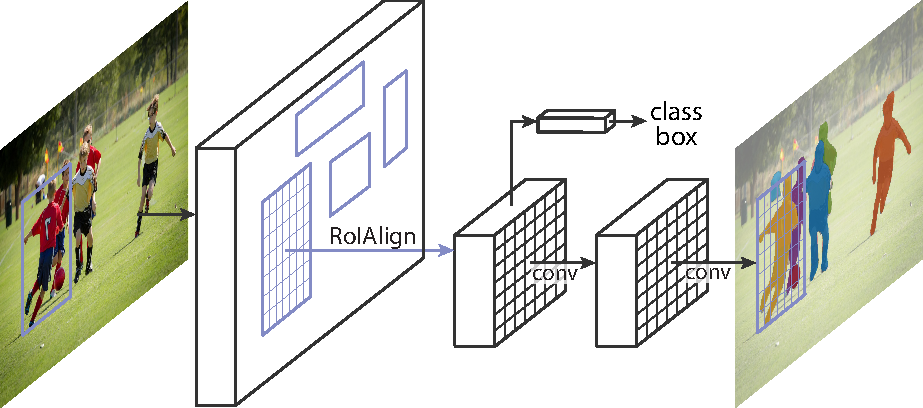
\includegraphics[width=1\linewidth]{figures/mask_rcnn/teaser}\vspace{2mm}
  \caption{用于实例分割的\textbf{Mask\hspace{0.1297em}R-CNN}框架。}
  \label{fig:teaser}
\end{minipage}\hspace{1.5em}
\begin{minipage}{0.5\textwidth}
  \begin{minipage}{0.365\linewidth}
  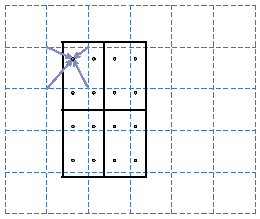
\includegraphics[width=\textwidth,trim={0 0 7.5mm 0},clip]{figures/mask_rcnn/roialign}
  \end{minipage}\hspace{0.5em}
  \begin{minipage}{0.605\linewidth}
  \caption{\textbf{RoIAlign:} 虚线网格表示特征图,实线表示 RoI(在这个例子里面包含$2\times2$的容器),容器中的点表示每个容器中的4个采样点。RoIAlign通过特征图上附近网格点的双线性插值计算每个采样点的值。 在 RoI 内部,其容器或采样点中涉及的任何坐标都不执行量化。}
  \label{fig:roialign}
  \end{minipage}
\end{minipage}
\end{figure}

实例分割非常具有挑战性,因为它需要在正确地检测出一张图片中所有目标的同时,精确地划分每一个实例物体。因此实例分割问题包含了传统计算机视觉领域中的\emph{目标检测}和\emph{语义分割}任务。其中目标检测的任务是对于图片中的每一个目标进行分类,并使用边界框定位目标。而语义分割的目标是将图片中的每一个像素分类为一些固定的类别,而不区分每一个目标实例。\footnote{我们使用术语\emph{目标检测}表示检测目标的边界框,而不是遮罩;使用术语\emph{语义分割}表示将每一个像素分类而不区分目标实例,与通用的术语一致。同时我们使用术语\emph{实例分割}来表示既包含语义分割也包含目标检测的任务。} 对于实例分割任务,有人可能会认为需要一个复杂的方法才能得到好的结果。然而我们展示了一个极其简单、灵活以及快速的系统,能够超越先前在实例分割领域最先进的成果。

我们这个称为\emph{Mask R-CNN}的方法是Faster R-CNN的扩展,增加了一个用于预测每一个感兴趣区域(Region of Interest,RoI)的分割遮罩的分支,该分支与现有的用于分类及边界框回归的分支\emph{并行}(图~\ref{fig:teaser})。该遮罩分支是一个应用于每一个感兴趣区域的全连接卷积网络,用于像素到像素级别的分割遮罩预测。Faster R-CNN框架便于用很多种灵活的架构设计实现,对于一个特定的Faster R-CNN网络,基于此的Mask R-CNN模型很也容易实现和训练。不仅如此,遮罩分支仅增加了少量的计算量,使得一个快速的系统和实验成为可能。

Mask R-CNN的原则是作为Faster R-CNN的一个直观的扩展框架,然而正确地构造遮罩分支是取得好结果的关键。更重要的是,Faster R-CNN不是为在输入和输出之间像素到像素对齐而设计的。这种设计在\emph{RoIPool}运用粗粒度的空间量化进行特征提取时最为明显。其中RoIPool是\emph{事实上的}处理实例的核心操作。为了解决不对齐的问题,我们提出了简单、免量化的层,称为\emph{RoIAlign},其完整地保留了额外的空间位置。尽管这看上去是一个很小的改变,然而具有很大的影响:它将遮罩预测的准确率相对提升了10\%到50\%,并且在更严格的评估方式下提升更明显。我们的第二个发现是,有必要将遮罩预测与分类预测\emph{解耦}:我们独立地对每个类别进行二元遮罩预测,取消了不同类别之间的竞争,同时利用网络中RoI分类分支进行类别预测。与之相反的,全卷积网络通常用于对每个像素进行多分类操作,该操作将分割与分类耦合起来,这样的传统方法在我们的实验的实例分割任务中表现不佳。

在没有使用任何调参技巧的情况下,Mask R-CNN的表现超过了所有先前在COCO实例分割任务中最优秀的单模型的结果,包括依靠高度工程化技巧赢得2016年挑战的冠军。作为一个附带的结果,我们的方法在COCO目标检测任务中依然表现出色。在控制变量分析对比实验中,我们评估了模型中多个基本的组成部分,这让我们能够评估模型的稳健性以及分析核心元素的影响。

我们的模型在单张GPU上每一帧的运行时间大约为200毫秒,在一台拥有8张GPU的机器上使用COCO数据集进行训练大约需要花费两天。我们相信如此快的训练和测试速度,以及模型的灵活性和准确性,能够让今后的实例分割研究获益。

最后,我们通过利用COCO姿势关键点数据库完成人类姿势估计任务简单展示了该框架的通用性。通过将每一个关键点看作是一个有固定个数1的二元遮罩,再加上一些很小的修改,就可以将原始的Mask R-CNN框架应用于检测每一个人物实例的姿势。在没有任何调参技巧的情况下,Mask R-CNN的表现超过了COCO 2016人物姿势关键点挑战的获胜者,同时检测速度依然是每秒5帧。因此Mask R-CNN可以更宽泛地看作是一个用于\emph{实例级别}的识别的灵活框架,并且可以很轻易地扩展到其它的复杂任务当中。

我们已经将源代码公开以促进今后的研究工作。

\xjtuappendixsection{相关工作}

\paragraph{R-CNN:} 基于区域的卷积神经网络(Region-based CNN,R-CNN)这样的用于边界框目标检测的方法,通常被用于处理大量的目标候选区域,同时独立地在每一个RoI上评估卷积网络。在2014年,经过扩展的R-CNN可通过RoIPool用于处理在特征图上的RoI,使其取得更高的准确率和更快的速度。Faster R-CNN再度扩展了此项工作,其使用区域候选网络(Region Proposal Network,RPN)来学习注意力机制。Faster R-CNN相比于之后的改进模型更加灵活和稳健 ,同时其依然是当前多个评估标准中领先的框架。

\paragraph{实例分割:} 受R-CNN良好效果的影响,很多实例分割的方法都是基于\emph{分割候选物}的。先前的方法  都采取的是自下而上的分割形式 . DeepMask  以及接下来的工作  会通过学习生成分割形状的候选,这些候选将使用Fast R-CNN进行分类。在这些方法中,形状的分割\emph{先于}目标的识别,这种做法不仅速度慢,而且精度低。类似地,戴先生等人  提出了一个复杂的多级级联,该方法在分类之后使用候选的边界框来预测候选的分割形状。与此相反,我们的方法基于\emph{并行的}遮罩和类别预测任务,使得该方法更加简单和灵活。

最近,李先生等人  将中的候选分割形状系统与中的目标检测系统结合起来,用于 ``全卷积实例分割'' (fully convolutional instance segmentation,FCIS)。 在  当中的基本想法是预测一系列全卷积的且位置敏感的输出通道。这些通道可同时呈现目标类别、边界框以及遮罩信息,使得系统更快。但是 FCIS 也暴露了其在重叠的实例上会出现系统性的错误,以及会生成一些假的遮罩边缘(见图~\ref{fig:results_vs_fcis}),这表明了在实例分割问题上存在根本性的困难,极具挑战性。

其它形式的实例分割解决方案  是由语义分割问题的解决来驱动的。由每一个像素的分类结果出发(例如FCN的输出),这些方法尝试将同一个类别的像素分割为不同的实例。与这些方法中\emph{分割优先}策略相反,Mask R-CNN基于\emph{实例优先}的策略。我们期待在今后的研究中,两种策略可以更进一步地融合。

\xjtuappendixsection{Mask R-CNN}\label{sec:maskR-CNN}

Mask R-CNN 在概念上很简洁:Faster R-CNN对于每个候选的目标会有两个输出,一个是目标的分类标签,另一个是目标的边界框。基于此我们增加了第三个分支,用于输出目标的遮罩。因此Mask R-CNN是一个自然而直观的想法。然而增加的遮罩输出与类别标签和边界框输出不同,需要获取一个目标更\emph{细致}的空间分布信息。接下来我们将介绍Mask R-CNN的关键元素,这些元素是Fast/Faster R-CNN所缺少的。

\paragraph{Faster R-CNN:} 我们首先简单回顾一下Faster R-CNN检测器 。Faster R-CNN 包含两个阶段。第一个阶段称为区域候选网络(Region Proposal Network,RPN),该阶段生成候选的目标边界框。第二个阶段本质上是一个Fast R-CNN 模型, 该阶段使用RoIPool从每一个候选框中提取特征,将这些特征用于分类和边界框回归。两个阶段使用的特征可以共享,以此来加速检测的速度。我们建议读者阅读以了解Faster R-CNN与其它框架最新的、最全面的对比。

\paragraph{Mask R-CNN:} Mask R-CNN同样包含两个阶段的过程,并且第一阶段(RPN)没有改动。在第二阶段,在\emph{并行}地预测类别标签和边界框两条分支的同时,Mask R-CNN对于每一个RoI还输出了一个二元的遮罩。这与最近出现的系统相反,在那些系统中分类\emph{独立于}遮罩预测(例如 )。我们的方法继承Fast R-CNN 的精神,将边界框的分类和回归\emph{并行}执行,这种精神已经被证实大量简化了原始的R-CNN 中多阶段流水线过程。

形式化的表述是,在训练阶段,我们在每一个采样的RoI上定义了一个多任务的损失函数,该损失函数表示为$L = L_{cls} + L_{box} + L_{mask}$。其中分类损失 $L_{cls}$ 和边界框损失 $L_{box}$ 与当中的定义相一致。遮罩分支对于每一个RoI都有一个$Km^2$维的输出,该输出由$K$个分辨率为$m \times m$的二元遮罩组成,每一个遮罩对应于$K$个类别当中的一个类别。为了达到这样的目标,我们对每一个像素都使用了sigmoid函数激活,同时定义$L_{mask}$为平均二元交叉熵损失。对于真实分类标签为$k$的RoI,$L_{mask}$只由第$k$个遮罩定义(输出的其它遮罩不参与损失的计算)。

我们这样定义的 $L_{mask}$ 允许网络为每一个类别都生成一个遮罩,避免了不同类别之间遮罩的影响。我们依赖一个独立的分类分支来预测分类,分类结果用于从遮罩输出当中选择一个。这样使得遮罩分支与分类分支\emph{解耦}。与通常的实践不同得是,在通常的实践中,FCN会被用于语义分割,且通常会使用针对每一个像素的\emph{sigmoid}函数,以及\emph{多项的}交叉熵损失。在这样的情况下,不同类别的遮罩会存在冲突,而在我们的方法中不会这样,因为我们使用了针对每一个像素的 \emph{sigmoid}函数以及\emph{二元}损失。我们通过实验证明了这样的形式是我们取得好的实例分割结果的关键。

\paragraph{遮罩的表示:} 一个遮罩编码了一个输入目标的\emph{空间上的}布局。因此,不像类别标签以及边界框这样必须通过全连接层(\emph{fc})降维成短向量,提取遮罩的空间结构可以很自然地想到利用卷积来表达像素到像素之间的相关性。

特别地,我们使用 FCN  对于每一个RoI预测了一个尺寸为$m \times m$的遮罩。这使得遮罩分支内的每一层保留明确的$m \times m$的目标物体空间布局,而非将其折叠成一个缺少空间信息的向量。与先前采取全连接(\emph{fc})层来预测遮罩的方法 ,我们的全卷积表示需要的参数更少,并且实验表明这样的准确率更高。

这种像素到像素的行为要求我们的 RoI 特征(它们本身就是小特征图)能够很好地对齐,从而忠实地保留显式的每像素空间相关性。这促使我们开发了以下 \emph{RoIAlign} 层,该层在遮罩预测中发挥关键作用。

\paragraph{RoIAlign:} RoIPool  是从每个 RoI 中提取一个小特征图(例如~$7\times7$)的标准操作。 RoIPool 首先将由浮点数构成的RoI\emph{量化}为离散粒度的特征图,然后将该量化的RoI划分为自身量化的空间容器,最后聚合每个容器所涵盖的特征值(通常通过最大池化)。例如对于连续坐标 $x$, 量化是通过计算 $x / 16$来执行的,其中 16 是特征图的步长,$[\cdot]$是舍入;同样地,当划分容器(例如~$7\times7$)时执行的也是量化。 这些量化引入了 RoI 和提取的特征之间的错位。 虽然这可能不会影响分类,这对于小型的转换很有用,但它对预测精确到像素级别的遮罩有很大的负面影响。

为了解决这个问题,我们提出一个\emph{RoIlign}层,其去除了RoIPool层的严格量化,正确地将提取的特征与输入\emph{对齐}。 我们提出的修改很简单:我们避免任何RoI边界或容器的量化(例如,我们使用$x/16$而不是$[x/16]$)。 我们使用双线性插值计算每个RoI容器中四个常规采样位置的输入特征的精确值,并汇总结果(使用最大值或平均值),详细信息请参见图\ref{fig:roialign}。我们注意到,结果对精确的采样位置,或者对有多少个点进行采样不敏感,\emph{只要}不进行量化即可。

正如我们在\S 附录\ref{sec:ablations}中所示,RoIAlign可以带来很大的改进。我们也比较了RoIWarp提出的操作。与RoIAlign不同,RoIWarp忽略了对齐问题,并像RoIPool一样实现了量化RoI。因此,尽管RoIWarp也采用了双线性重采样,但它的性能与RoIPool相当(如表\ref{tab:ablation:roialign}所示),证明了对齐的关键作用。

\paragraph{网络体系结构:} 为了演示我们方法的一般性,我们实例化了具有多种体系结构的Mask R-CNN。为了清楚起见,我们区分:(i)用于整个图像上的特征提取的卷积\emph{主干}体系结构,以及(ii)用于边界框识别(分类和回归)的网络\emph{前部}和分别应用于每个RoI的遮罩预测。

我们用术语\emph{网络深度特征}来表示主干体系结构。 我们评估深度为50或101层的ResNet和ResNeXt 网络。带有ResNet的Faster R-CNN的最初实现从第四阶段的最后卷积层提取特征,我们称之为C4。 例如,ResNet-50 的主干用 ResNet-50-C4 表示。 这是一个常用的表示选择和表示方式。

我们还探索了林先生等人最近提出的另一种更有效的主干网络,称为特征金字塔网络(Feature Pyramid Network,FPN)。 FPN 使用具有横向连接的自顶向下架构从单一比例输入构建网络内特征金字塔。以FPN为主干的Faster R-CNN根据其规模从不同层次的特征金字塔中提取 RoI 特征,但其他方法与 vanilla ResNet 类似。以ResNet-FPN为主干的Mask R-CNN进行特征提取可以提高精度和速度。有关FPN的更多详细信息,请读者参阅相关文献。

对于网络的\emph{前部},我们大部分沿用以前工作中提出的架构,并在其中添加全卷积遮罩预测分支。具体来说,我们根据ResNet和FPN论文扩展了Faster R-CNN的前部。 详细信息如图\ref{fig:head}所示。 ResNet-C4主干的前部包括计算密集的ResNet第5阶段(即9层的`res5')。对于FPN,主干已经包含 res5,因此允许使用更少卷积核的更高效的前部。

我们注意到我们的遮罩分支有一个简单的结构。更复杂的设计有提高性能的潜力,但不是这项工作的重点。

\begin{figure}[t]
\centering
\begin{overpic}[width=1.0\linewidth]{figures/mask_rcnn/head}
 \put(33,29){\tiny Faster R-CNN}
 \put(33,27){\tiny w/ ResNet }
 \put(84,29){\tiny Faster R-CNN}
 \put(85,27){\tiny w/ FPN }
\end{overpic}
\caption{\textbf{前部体系结构}: 我们扩展了两个现有的Faster R-CNN的前部。 左图和右图分别显示ResNet C4和FPN主干的前部,其都添加了遮罩分支。数字表示空间分辨率和通道数。箭头表示可以从上下文中推断出的卷积层、反卷积层或者全连接层(卷积层会保留空间维度,而反卷积层会增加空间维度)。除了输出卷积层的尺寸为$1\times1$,所有的卷积核的尺寸都是$3\times3$。反卷积核尺寸为$2\times2$且步长为2,同时我们在隐藏层中使用了ReLU。 \emph{左}:`res5'表示ResNet的第五阶段,为了简单起见,我们进行了更改,使得第一个卷积核以步长1在尺寸为$7\times7$的RoI上操作,(而不是以步长2在尺寸为$14\times14$RoI上)。\emph{右}:$\times4$表示一连串的四次转换。}
\label{fig:head}
\end{figure}

\xjtuappendixsubsection{实现细节}\label{sec:impl}

我们根据现有的Fast/Faster R-CNN工作来设置超参数。尽管这些超参数的设置是针对原始论文中的目标检测任务而做出的,但我们发现这些设置对于我们的实例分割任务也是健壮的。

\paragraph{训练:} 与Fast R-CNN一样,如果RoI的与真实边界框的IoU大于或等于0.5,则RoI被认为是正确的,否则为错误的。遮罩损失$L_{mask}$仅在正确的RoI上定义。遮罩的目标输出是正确的RoI与其关联的实际遮罩之间的交集。

\begin{figure*}[t]
\centering
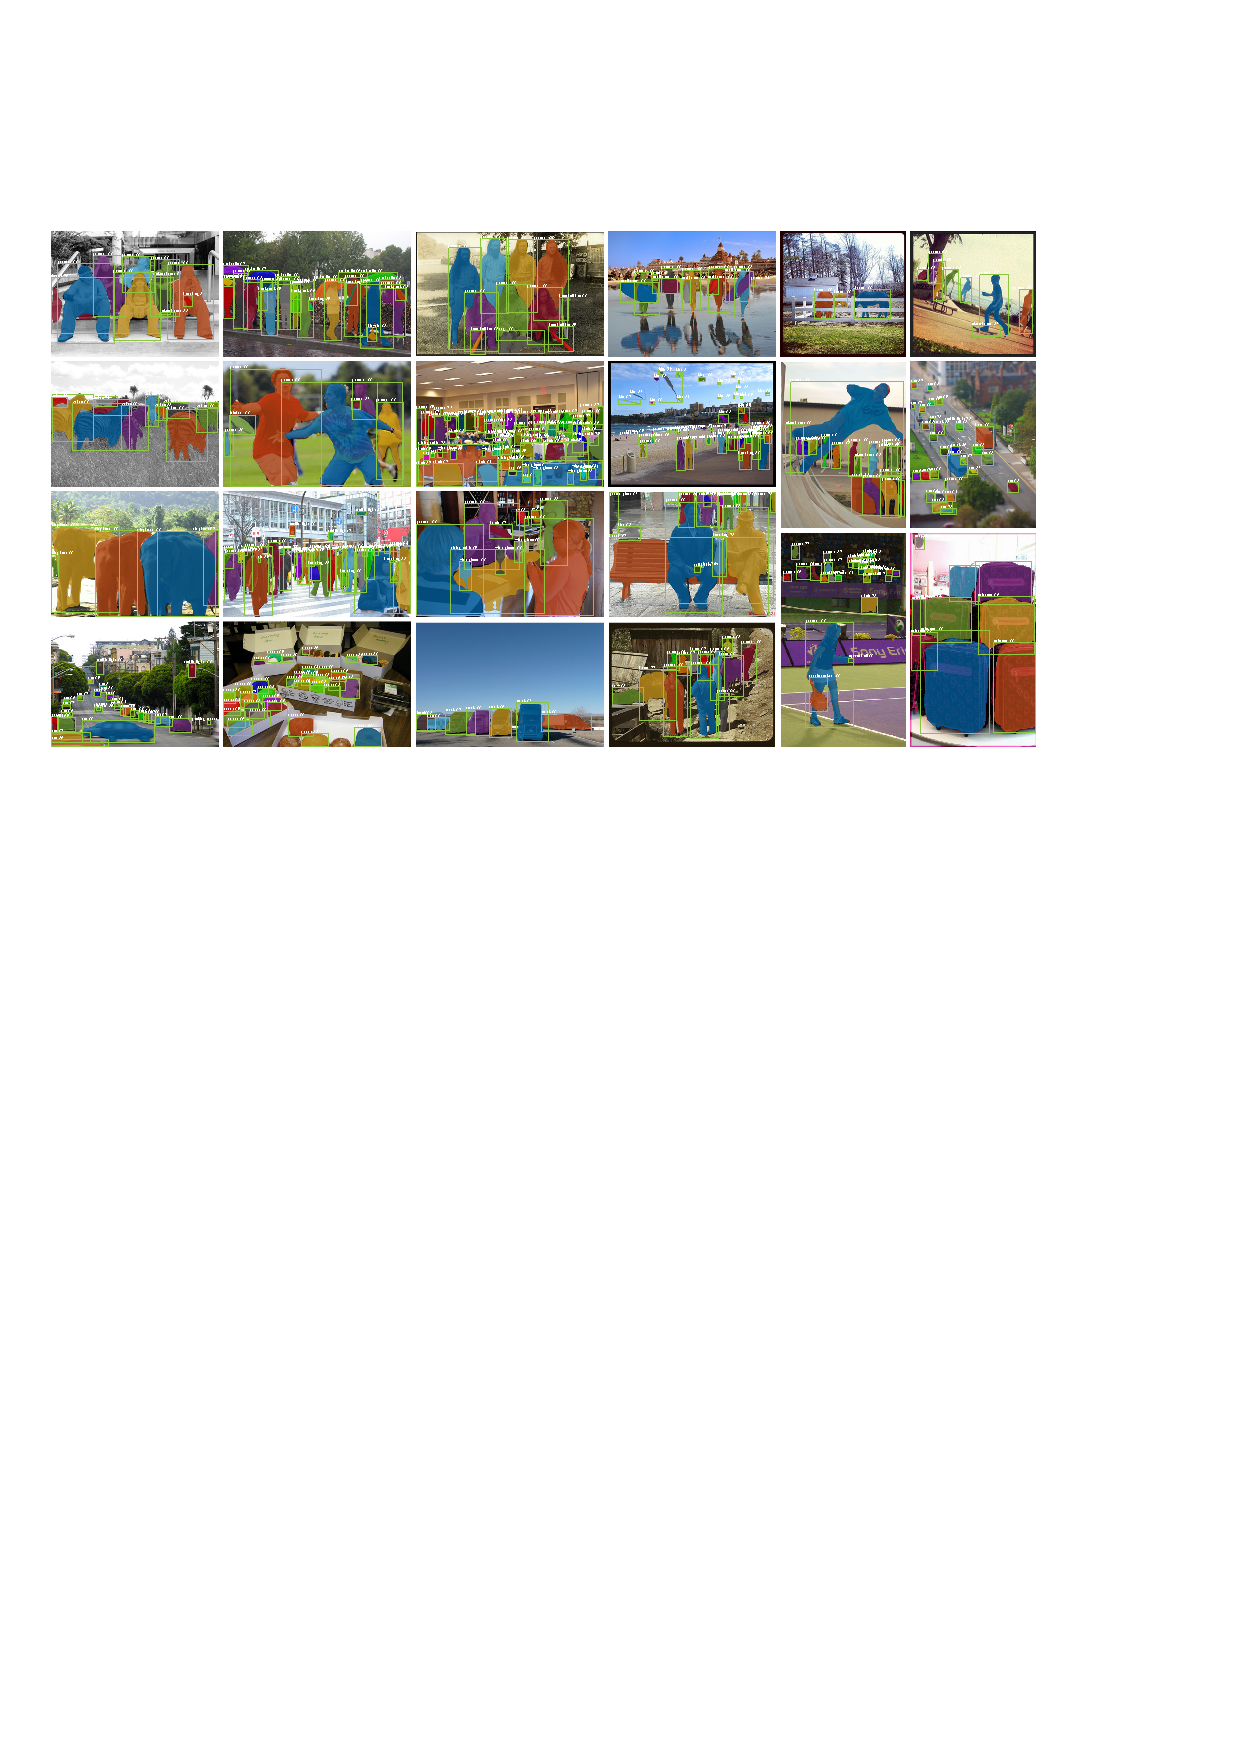
\includegraphics[width=1.0\linewidth]{figures/mask_rcnn/results_more}
\caption{\textbf{Mask R-CNN}在COCO测试集上的更多结果。取得该结果的模型使用了ResNet-101-FPN作为主干,速度为5fps,遮罩平均精度为35.7(见表\ref{tab:final_mask})。}
\label{fig:results_more}
\end{figure*}

\begin{table*}[t]
\tablestyle{3.5pt}{1.1}
\begin{tabular}{l|l|x{22}x{22}x{22}|x{22}x{22}x{22}}
 & backbone &  AP &  AP$_{50}$ & AP$_{75}$ & AP$_S$ &  AP$_M$ &  AP$_L$\\
\shline
 MNC  & ResNet-101-C4
  & 24.6 & 44.3 & 24.8 & 4.7 & 25.9 & 43.6\\
 FCIS  +OHEM & ResNet-101-C5-dilated
  & 29.2 & 49.5 & - & 7.1 & 31.3 & 50.0\\
 FCIS+++  +OHEM & ResNet-101-C5-dilated
  & 33.6 & 54.5 & - & - & - & -\\
\hline
 \bd{Mask R-CNN} & ResNet-101-C4
  & 33.1 & 54.9 & 34.8 & 12.1 & 35.6 & 51.1 \\
 \bd{Mask R-CNN} & ResNet-101-FPN
  & 35.7 & 58.0 & 37.8 & 15.5 & 38.1 & 52.4\\
 \bd{Mask R-CNN} & ResNeXt-101-FPN
  & \bd{37.1} & \bd{60.0} & \bd{39.4} & \bd{16.9} & \bd{39.9} & \bd{53.5}
\end{tabular}
\caption{\textbf{实例分割} 在COCO\texttt{test-dev}数据集上的\emph{遮罩}平均精度. MNC和FCIS分别是2015年和2016年COCO实例分割挑战的获胜者。在没有任何调参技巧的情况下,Mask R-CNN的表现超过了更复杂的FCIS+++模型,该模型包括了多尺度训练、测试,水平平移测试,以及OHEM。所有的图片都是\emph{单一模型}下的结果。}
\label{tab:final_mask}
\end{table*}

我们采用图像中心训练。调整图像大小以使其长、宽中较短的一边为800像素。每个最小批量在每个GPU上有2张图像,每个图像都有$N$个抽样的RoI,比例为1:3。在C4主干下,$N$为64,在FPN主干下,$N$为512。我们在8个GPU上进行训练(因此有效的最小批量为16),进行16万次迭代,学习率为0.02,在迭代12万次时减少为原来的$1/10$。我们使用0.0001作为重量衰减以及0.9作为动量。在使用使用ResNeXt时,我们每个GPU训练1个图像并进行相同次数的迭代,初始学习率为0.01。

RPN锚点(anchors)跨越5个尺度和3个纵横比。为了方便控制变量,除非另有说明,否则RPN将单独进行训练并且不与Mask R-CNN共享特征。对于本文中的每个部分,RPN和Mask R-CNN具有相同的主干,因此它们的参数可以共享。

\paragraph{预测:} 在测试时,以C4为的候选框个数为300,以FPN为主干的候选框个数为1000。我们将这些候选框分别送入边界框预测分支,然后进行非最大抑制。然后将得分最高的100个检测框输入遮罩分支。虽然这与训练中使用的并行计算不同,但它加快了预测速度并提高了准确性(因为使用了更少,更准确的RoI)。遮罩分支对于每个RoI可以预测$k$个遮罩,但我们只使用第$k$个遮罩,其中$k$是分类分支预测的类别。然后将尺寸为$m\times m$的浮点数遮罩输出调整为RoI的大小,并使用阈值0.5将其二值化。

请注意,由于我们仅在前100个检测框中计算掩码,因此Mask R-CNN相对其对应的Faster R-CNN模型进增加了一个很小的开销(例如在典型模型上大约为20\%)。

\xjtuappendixsection{实验:实例分割}\label{sec:results}

我们在COCO数据集上以控制变量的方式,将Mask R-CNN与对应领域最先进的模型进行了彻底的比较。我们展示COCO数据集上常规的指标,包括平均精度(AP,在IoU阈值以上的均值),$AP_{50}$,$AP_{75}$和$AP_S$,$AP_M$,$AP_L$(不同AP规模)。除非另有说明,AP将使用\emph{遮罩}IoU进行评估。与以前的工作一样,我们使用8万张训练图像和3.5万张验证集子集图像(\texttt{trainval35k})进行训练,并展示剩余的5千张验证集图像(\texttt{minival})上的控制变量实验。我们还展示了\texttt{test-dev}测试集上的结果。

\xjtuappendixsubsection{主要结果}

\begin{figure*}[t]
\centering
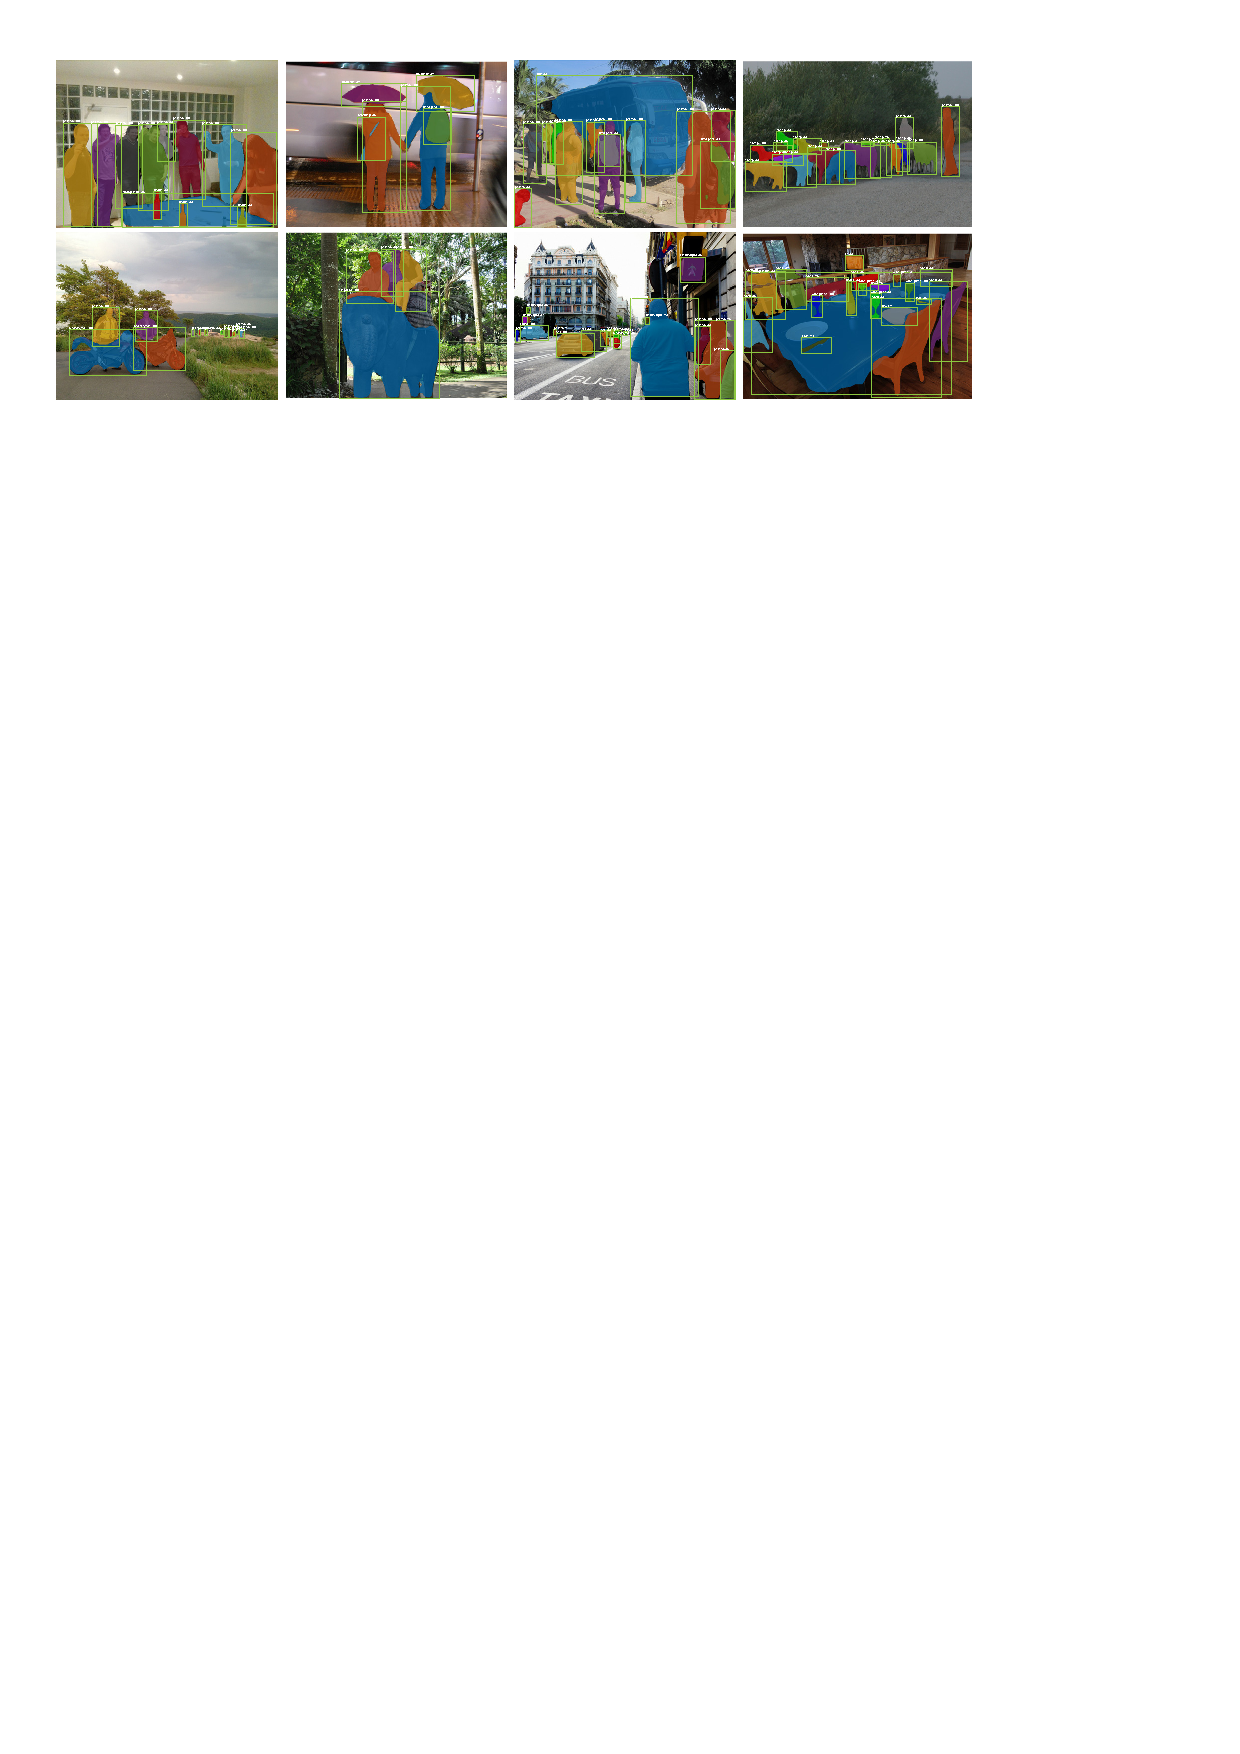
\includegraphics[width=1\linewidth]{figures/mask_rcnn/results_main}
\caption{\textbf{Mask R-CNN}框架在COCO测试集上的结果。这些结果基于ResNet-101  模型,达到了35.7的\emph{遮罩}准确率,且运行速度为每秒5帧. 遮罩使用了不同的颜色来展示。图中同样展示了边界框、类别名称以及置信度。}
\label{fig:results_main}\vspace{-2mm}
\end{figure*}

我们将Mask R-CNN与最先进的实例分割模型进行比较,结果如图\ref{tab:final_mask}。我们模型的所有实例都优于先前最先进的模型的基础变体。这包括MNC和FCIS,它们分别是2015年和2016年的分类挑战的获胜者。以ResNet-101-FPN为主干的Mask R-CNN无需任何调参技巧,就胜过FCIS+++模型,该模型包括多尺度训练、测试,水平翻转测试和在线硬模式挖掘(OHEM)。虽然超出了本工作的范围,但我们预计将会有很多在我们此工作上的改进。

Mask R-CNN的输出可视化为图\ref{fig:results_main}和图\ref{fig:results_more}。Mask R-CNN即使在具有挑战性的问题下也能取得良好效果。在图\ref{fig:results_vs_fcis}中,我们比较了我们的Mask R-CNN基础模型和FCIS+++。FCIS+++在重叠的实例中显示了系统性的错误,表明它受到实例分割的根本难度的挑战。Mask R-CNN没有显示出这样的错误。

\begin{figure*}[t]
\centering
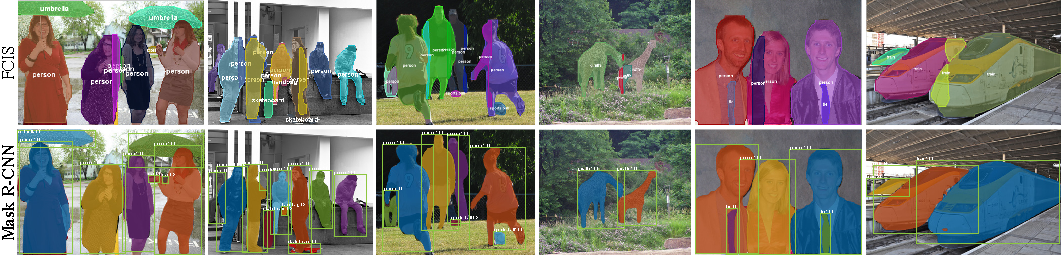
\includegraphics[width=1.0\linewidth]{figures/mask_rcnn/results_vs_fcis}
\caption{FCIS+++(上) 对比 Mask R-CNN(下, 以ResNet-101-FPN为主干). FCIS在重叠的实例中显示了系统性的错误。}
\label{fig:results_vs_fcis}
\end{figure*}

\begin{table*}[t]
% subfloat a - BackBone Architecture
\subfloat[\textbf{主干模型体系结构}: 更好的主干模型带来预期的收益:更深的网络效果更好,FPN优于C4特征,ResNeXt改进了ResNet。\label{tab:ablation:backbone}]{
\tablestyle{2.5pt}{1.05}\begin{tabular}{c|x{22}x{22}x{22}}
 \scriptsize \emph{net-depth-features} & AP & AP$_{50}$ & AP$_{75}$\\
\shline
 \scriptsize ResNet-50-C4 & 30.3 & 51.2 & 31.5\\
 \scriptsize ResNet-101-C4 & 32.7 & 54.2 & 34.3\\\hline
 \scriptsize ResNet-50-FPN & 33.6 & 55.2 & 35.3\\
 \scriptsize ResNet-101-FPN & 35.4 & 57.3 & 37.5\\
 \scriptsize ResNeXt-101-FPN & \bd{36.7} & \bd{59.5} & \bd{38.9}
\end{tabular}}\hspace{1mm}
% subfloat b - Multinomial vs Independent Masks
\subfloat[\textbf{耦合的对比解耦的遮罩分支} (ResNet-50-C4): 通过每个类别的二元遮罩\emph{解耦}相比于耦合的遮罩预测有了很大提升。\label{tab:ablation:sigmoid}]{
\tablestyle{4.8pt}{1.05}\begin{tabular}{c|x{22}x{22}x{22}}
 & AP & AP$_{50}$ & AP$_{75}$\\
\shline
 \emph{softmax} & 24.8 & 44.1 & 25.1\\
 \emph{sigmoid} & \bd{30.3} & \bd{51.2} & \bd{31.5}\\
\hline
 & \dt{+5.5} & \dt{+7.1} & \dt{+6.4}\\
 \multicolumn{4}{c}{~}\\
 \multicolumn{4}{c}{~}\\
\end{tabular}}\hspace{1mm}
% subfloat c - RoIAlign (ResNet-50-C4)
\subfloat[\textbf{RoIAlign} (ResNet-50-C4): 用各种RoI图层的遮罩预测结果。我们的RoIAlign层使平均精度提高了3个百分点,AP$_{75}$大约提高了5个百分点。使用适当的对齐是影响RoI层之间巨大差距的唯一因素。\label{tab:ablation:roialign}]{
\tablestyle{2.2pt}{1.05}\begin{tabular}{c|c|c|c|x{22}x{22}x{22}}
 & \scriptsize\textbf{align?} & \scriptsize bilinear? & \scriptsize agg.
 & AP & AP$_{50}$ & AP$_{75}$\\
\shline
 \emph{RoIPool}
  & & & max & 26.9 & 48.8 & 26.4\\
\hline
 \multirow{2}{*}{\emph{RoIWarp} }
  & & \checkmark & max & 27.2 & 49.2 & 27.1\\
  & & \checkmark & ave & 27.1 & 48.9 & 27.1\\
\hline
 \multirow{2}{*}{\emph{RoIAlign}}
  & \checkmark & \checkmark & max & \bd{30.2} & \bd{51.0} & \bd{31.8}\\
  & \checkmark & \checkmark & ave & \bd{30.3} & \bd{51.2} & \bd{31.5}
\end{tabular}}\\
% subfloat d - RoIAlign (ResNet-50-C5)
\subfloat[\textbf{RoIAlign} (ResNet-50-\bd{C5}, \emph{stride 32}): 使用大步长特征的遮罩任务和边界框任务的平均精度。错位比步长为16的特征更严重(表\ref{tab:ablation:roialign}),导致较大的精度差距。\label{tab:ablation:roialign32}]{
\tablestyle{4pt}{1.05}\begin{tabular}{c|x{22}x{22}x{22}|x{22}x{22}x{22}}
 & AP & AP$_{50}$ & AP$_{75}$
 & AP$^\text{bb}$ & AP$^\text{bb}_{50}$ & AP$^\text{bb}_{75}$ \\[.1em]
\shline
 \emph{RoIPool} & 23.6 & 46.5 & 21.6 & 28.2 & 52.7 & 26.9\\
 \emph{RoIAlign} & \bd{30.9} & \bd{51.8} & \bd{32.1} & \bd{34.0} & \bd{55.3} & \bd{36.4}\\
\hline
 & \dt{+7.3} & \dt{+ 5.3} & \dt{+10.5} & \dt{+5.8} & \dt{+2.6} & \dt{+9.5}
\end{tabular}}\hspace{5mm}
% subfloat e - mask representation
\subfloat[\textbf{遮罩分支 } (ResNet-50-FPN): 全卷积网络(FCN)对比多层感知机(MLP,全连接的)用于遮罩预测。FCN改善了结果,因为它们利用了明确编码的空间布局的优势。\label{tab:ablation:maskhead}]{
\tablestyle{4pt}{1.05}\begin{tabular}{c|c|x{22}x{22}x{22}}
 & mask branch & AP & AP$_{50}$ & AP$_{75}$\\
\shline
 MLP & fc: 1024$\rightarrow$1024$\rightarrow$$80\ncdot28^2$  & 31.5 & 53.7 & 32.8\\
 MLP & fc: 1024$\rightarrow$1024$\rightarrow$1024$\rightarrow$$80\ncdot28^2$ & 31.5 & 54.0 & 32.6\\
\hline
 \textbf{FCN} &  conv: 256$\rightarrow$256$\rightarrow$256$\rightarrow$256$\rightarrow$256$\rightarrow$80
 & \bd{33.6} & \bd{55.2} & \bd{35.3}
\end{tabular}}
% main caption
\caption{\textbf{对比试验}。我们在\texttt{trainval35k}上训练,在\texttt{minival}上测试。除非特别说明,以上都是\emph{遮罩}平均精度指标。}
\label{tab:ablations}
\end{table*}

\xjtuappendixsubsection{控制变量对比试验}\label{sec:ablations}

我们对Mask R-CNN进行了一系列的控制变量对比实验分析。结果显示在表\ref{tab:ablations}中并在下面详细讨论。

\paragraph{体系结构:} 表\ref{tab:ablation:backbone}展示了Mask R-CNN在不同的主干模型下的结果。Mask R-CNN受益于更深的网络(50层对比101层)和先进的设计,包括FPN和ResNeXt。 我们注意到\emph{不是}所有框架都会自动从更深或更高级的网络中受益。

\paragraph{耦合的和解耦的遮罩分支:} Mask R-CNN将遮罩预测和类别预测\emph{解耦}:现有的边界框分支已经可以预测类别标签,因此我们为每个类别生成一个遮罩,而不会造成类别的冲突(由于每个像素的\emph{sigmoid}函数和\emph{二元}损失)。 在表\ref{tab:ablation:sigmoid}中,我们将其与对每个像素进行\emph{softmax}激活和多项损失(如FCN中常用的)进行比较。这种替代方案将遮罩和类别预测任务相\emph{耦合},并导致遮罩平均精度下降了5.5个百分点。 这表明,一旦实例被整体分类(通过边界框分支),就足够预测二元遮罩了,而不用考虑类别,这使得模型更易于训练。

\paragraph{类别已知和类别不可知的遮罩预测:} 我们默认的实例化模型是在类别已知的情况下进行遮罩预测的。例如对于每一个类别,都会预测一个$m\times m$的遮罩。有趣的是,在类别不可知的情况下(例如无论类别如何,只输出一个$m\times m$的遮罩),Mask R-CNN几乎同样有效:其取得了29.7的遮罩均值精度,相比于类别已知模型30.3的均值精度,它们都是以ResNet-50-C4为主干模型。这进一步突出了我们的方法中的分工,这在很大程度上使得分类任务和分割任务解耦。

\begin{table*}[t]
\tablestyle{3.5pt}{1.1}
\begin{tabular}{l|l|x{22}x{22}x{22}|x{22}x{22}x{22}}
 & backbone
 & AP$^\text{bb}$ & AP$^\text{bb}_{50}$ & AP$^\text{bb}_{75}$
 & AP$^\text{bb}_S$ & AP$^\text{bb}_M$ &  AP$^\text{bb}_L$\\ [.1em]
\shline
 Faster R-CNN+++  & ResNet-101-C4
  & 34.9 & 55.7 & 37.4 & 15.6 & 38.7 & 50.9\\
 Faster R-CNN w FPN  & ResNet-101-FPN
  & 36.2 & 59.1 & 39.0 & 18.2 & 39.0 & 48.2\\
 Faster R-CNN by G-RMI  & Inception-ResNet-v2
  & 34.7 & 55.5 & 36.7 & 13.5 & 38.1 & 52.0\\
 Faster R-CNN w TDM  & Inception-ResNet-v2-TDM
  & 36.8 & 57.7 & 39.2 & 16.2 & 39.8 & \bd{52.1}\\
\hline
  Faster R-CNN, RoIAlign & ResNet-101-FPN
  & 37.3 & 59.6 & 40.3 & 19.8 & 40.2 & 48.8\\
 \bd{Mask R-CNN} & ResNet-101-FPN
  & 38.2 & 60.3 & 41.7 & 20.1 & 41.1 & 50.2\\
 \bd{Mask R-CNN} & ResNeXt-101-FPN
  & \bd{39.8} & \bd{62.3} & \bd{43.4} & \bd{22.1} & \bd{43.2} & {51.2}
\end{tabular}
\caption{\textbf{目标检测} \emph{单一模型} 的结果 (边界框均值精度), 对比该领域最先进的方法,在\texttt{test-dev}测试集上. 使用ResNet-101-FPN作为主干模型的Mask R-CNN的表现超过了所有先前该领最先进的模型的基础变种(在这个任务中,遮罩预测输出会被直接忽略)。Mask R-CNN相对于Faster R-CNN的提升主要来自于使用了RoIAlign(+1.1 $AP^\text{bb}$)、多任务训练(+0.9 AP$^\text{bb}$)以及ResNeXt-101(+1.6 AP$^\text{bb}$)。}
\label{tab:final_bbox}
\end{table*}

\paragraph{RoIAlign:} 我们提出的\emph{RoIAlign}层的性能评估如表\ref{tab:ablation:roialign}所示。对于这个实验,我们使用了步长为16的ResNet-50-C4作为主干模型。RoIAlign相比于RoIPool在均值精度上提升了3个百分点,其中大部分收益来自高IoU(例如AP$_{75}$)。RoIAlign对最大池化或平均池化不敏感;我们在本文的其余部分均使用平均池化。

此外,我们与在MNC中提出的\emph{RoIWarp}做了比较,其同样采用了双线性采样。正如在\S\ref{sec:maskR-CNN}所讨论的,RoIWarp依然量化RoI,使得与输入不对齐。从表\ref{tab:ablation:roialign}可以看出,RoIWarp 的表现与RoIPool相当,但比RoIAlign差很多。这突出表明正确的对齐是很关键的。

我们还对以\emph{ResNet-50-C5}作为主干模型的RoIAlign进行了评估,该主干模型以更大的32像素作为步长。我们使用与图\ref{fig:head}(右)中相同的前部,因为res5与此不兼容。从表\ref{tab:ablation:roialign32}可看出,RoIAlign在均值精度上提升了7.3个百分点,在遮罩AP$_{75}$提升了10.5个百分点(\emph{50\%的相对提升})。更进一步地,我们注意到对于RoIAlign,使用\emph{stride-32} C5特征(30.9 AP)比使用stride-16 C4特征(30.3 AP, 表\ref{tab:ablation:roialign})更加精准。RoIAlignn 在很大程度上解决了使用大步长特征进行检测和分割的长期挑战。

最后,与FPN一起使用时,RoIAlign在遮罩均值精度上能得到1.5个百分点的提升,在边界框均值精度上得到0.1),RoIAlign即使使用FPN(表\ref{tab:roialign_keypoint})也显示出较大的提升。

\paragraph{遮罩预测分支:} 分割是像素到像素的任务,我们通过使用FCN来利用遮罩的空间布局。在表\ref{tab:ablation:maskhead}中,我们比较了多层感知机(MLP)和使用了ResNet-50-FPN作为主干模型的FCN。使用FCN相对于MLP在遮罩均值精度上提升了2.1个百分点。我们注意到,我们选择这个骨干,以便FCN前部的卷积层没有预先训练,以公平地与MLP比较。

\xjtuappendixsubsection{边界框检测结果}

我们将Mask R-CNN与表\ref{tab:final_bbox}中的最新 COCO \emph{边界框}目标检测进行了比较。对于这个结果,即使完整的Mask R-CNN模型被训练,只有分类和边界框输出用于预测(遮罩输出被忽略)。 使用ResNet-101-FPN的Mask R-CNN优于所有先前最先进的模型的基础变种,包括G-RMI的单一模型,其为COCO 2016目标检测挑战赛的获胜者。通过使用ResNeXt-101-FPN,Mask R-CNN 进一步提高了结果,与之前使用 Inception-ResNet-v2-TDM的最佳单一模型相比,边界框均值精度提升了3.0个百分点。

作为进一步的比较,我们训练了一个\emph{没有}遮罩预测分支的Mask R-CNN版本,在表\ref{tab:final_bbox}中记为``Faster R-CNN, RoIAlign''。由于RoIAlign的原因,该模型的表现要好于模型Faster R-CNN。另一方面,该模型比Mask R-CNN低0.9个百分点的均值精度。因此Mask R-CNN在边界框检测上的这种优势是由于多任务训练的带来好处。

最后,我们注意到Mask R-CNN在它的遮罩和边界框均值精度上有一个小的差距:例如,37.1(遮罩,表\ref{tab:final_mask})和39.8(边界框,表\ref{tab:final_bbox})之间的2.7个百分点。这表明我们的方法在很大程度上缩小了目标检测与更具挑战性的实例分割任务之间的差距。

\xjtuappendixsubsection{时间性能}

\paragraph{预测:} 我们在Faster R-CNN的4步训练之后训练一个在RPN和Mask R-CNN阶段共享特征的ResNet-101-FPN模型。在Nvidia Tesla M40 GPU上,该模型以每张图片195毫秒的速度运行(加上15m毫秒的CPU时间,将输出调整为原始分辨率),并实现了在统计意义上的与非共享模式相同的遮罩均值精度。我们还表示使用ResNet-101-C4的变体大约需要耗时400毫秒,因为其拥有一个计算任务更重的前部(图\ref{fig:head}),因此我们不推荐在实践中使用 C4 变体。

虽然Mask R-CNN速度很快,但我们注意到我们的设计并未针对速度进行优化,并且可以进一步改进以实现更好的速度和精确度折衷,例如,通过改变图像尺寸和候选框数量,不过这超出了本文的范围。

\paragraph{训练:} Mask R-CNN 的训练也很快。 在COCO\texttt{trainval35k}数据集上使用ResNet-50-FPN进行训练需要32小时的时间。我们同步使用8个GPU(每个最小批量有16张图像,耗时0.72秒)。若是训练ResNet-101-FPN则需要44个小时。 实际上,在\texttt{train}数据集上训练时,可以在\emph{一天之内}完成快速原型。我们希望这种快速训练能够消除该领域的一个主要障碍,并鼓励更多的人对这个具有挑战性的话题进行研究。

\begin{figure*}[t]
\centering
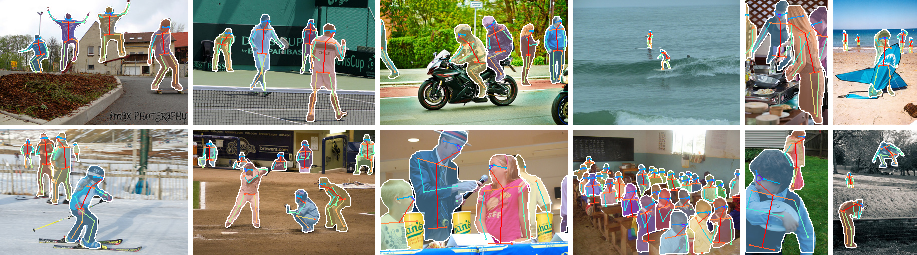
\includegraphics[width=1.0\linewidth]{figures/mask_rcnn/results_keypoints}
\caption{在COCO \texttt{test}数据集上使用Mask R-CNN(ResNet-50-FPN)进行关键点检测,包括从相同模型中预测出的人物分割遮罩。此模型的关键点均值精度为63.1,速度为每秒5张图片。}
\label{fig:results_keypoints}
\end{figure*}

\xjtuappendixsection{Mask R-CNN用于人体姿势估计}\label{sec:keypoints}

我们的框架可以很容易地扩展到人体姿态估计。我们将一个关键点的位置建模为二元遮罩,并采用Mask R-CNN来预测$K$个遮罩,每个遮罩用于表示$K$个关键点类型(例如,左肩,右肘)中的一个。这项任务有助于展示Mask R-CNN的灵活性。

我们注意到,我们的系统利用了人类姿态的\emph{最小}领域知识,因为实验主要是为了展示Mask R-CNN框架的通用性。我们期望领域知识(例如建模结构)会与我们简单的方法相辅相成。

\paragraph{实现细节:} 我们在将模型应用到对关键点预测时对分割系统进行了细微的修改。对于实例的$K$个关键点中的每个关键点,训练目标是二元$m\times m$的二进制遮罩,其中只有\emph{一个}像素被标记为前景。在训练期间,对于每个可见的真实关键点,我们将$m^2$路通过softmax输出(它鼓励单个点被检测到),并使用交叉熵损失进行最小化优化。我们注意到,与实例分割一样,$K$个关键点仍然是独立处理的。

我们采用了一个ResNet-FPN变体,其关键点前部结构与图\ref{fig:head}(右)相似。关键点前部由8个$3\times3$的、包含512个卷积核的卷积层组成,后面是去卷积层和2倍双线性放大,产生$56\times56$的输出分辨率。我们发现相对较高的分辨率输出(与遮罩分支相比)是关键点级别的定位精度所必需的。

模型在包含标注好关键点的COCO \texttt{trainval35k} 所有图像上进行训练。由于该训练集较小,为了减少过拟合,我们使用从 [640,800] 像素随机采样的图像进行训练。预测是在800像素的单一尺度上进行的。我们训练9万次迭代,从0.02的学习率开始,在6万和8万迭代时将其减少为当前的$1/10$。我们使用边界框NMS,阈值为0.5。其他细节与\S\ref{sec:impl}中的相同。

\begin{table}[t]
\tablestyle{1.8pt}{1.2}
\begin{tabular}{l|x{22}x{22}x{22}|x{22}x{22}}
 & AP$^\text{kp}$ & AP$^\text{kp}_{50}$ & AP$^\text{kp}_{75}$
 & AP$^\text{kp}_M$ &  AP$^\text{kp}_L$\\ [.1em]
\shline
CMU-Pose+++  & 61.8 & 84.9 & 67.5 & 57.1 & 68.2 \\
G-RMI $^\dagger$ & 62.4 & 84.0 & 68.5 & \bd{59.1} & 68.1 \\
\hline
 \bd{Mask R-CNN}, \footnotesize keypoint-only & 62.7 & 87.0 & 68.4 & 57.4 & 71.1 \\
 \bd{Mask R-CNN}, \footnotesize keypoint \& mask & \bd{63.1} & \bd{87.3} & \bd{68.7} & {57.8} & \bd{71.4} \\
\end{tabular}
\caption{\textbf{关键点检测} 在COCO \texttt{test-dev}数据集上的均值精度. 我们的模型是一个单一模型(ResNet-50-FPN),运行的速度为每秒5张图片。CMU-Pose+++ is 2016挑战的获胜者,其使用了多尺度测试,使用CPM进行后续处理,并且使用目标检测器进行过滤。我们的方法相比它提升了大约5个百分点(在个人通讯中声明)。$^\dagger$:G-RMI在COCO数据集\emph{以及}MPII数据集(2.5万张图片)上训练,使用两个模型(Inception-ResNet-v2用于边界框检测,ResNet-101用于关键点检测)。}
\label{tab:final_keypoint}
\end{table}

\paragraph{主要结果以及控制变量分析:}我们评估人体关键点的均值精度AP(AP$^\text{kp}$)并在实验中ResNet-50-FPN作为主干;附录中将研究更多主干模型。表\ref{tab:final_keypoint}显示我们的结果(62.7 AP$^\text{kp}$)比使用多级处理流水线的 COCO 2016关键点检测获胜者高0.9个百分点(请参阅表\ref{tab:final_keypoint}的标题)。我们的方法相当简单快捷。

\begin{table}[t]
\begin{minipage}{0.55\textwidth}
  \tablestyle{7pt}{1.1}
  \begin{tabular}{l|x{22}x{22}x{22}}
  & AP$^\text{bb}_\text{\emph{person}}$ & AP$^\text{mask}_\text{\emph{person}}$
  & AP$^\text{kp}$ \\ [.1em]
  \shline
  Faster R-CNN & 52.5 & - & - \\
  Mask R-CNN, mask-only & \bd{53.6} & \bd{45.8} & - \\
  Mask R-CNN, keypoint-only & 50.7 & - & 64.2 \\
  Mask R-CNN, keypoint \& mask & 52.0 & 45.1 & \bd{64.7} \\
  \end{tabular}
  \caption{对于\emph{人类}领域的边界框、遮罩以及关键点的\textbf{多任务学习},在\texttt{minival}数据集上的评估结果。所有的对比模型都使用相同的数据进行公平比较。主干模型是ResNet-50-FPN。在\texttt{minival}数据集上的均值精度为64.2和64.7模型在\texttt{test-dev}数据集上的均值精度分别为62.7和63.1(见表\ref{tab:final_keypoint})。}
  \label{tab:multitask_keypoint}
\end{minipage}\hspace{3mm}
\begin{minipage}{0.4\textwidth}
  \tablestyle{2pt}{1.1}
  \begin{tabular}{l|x{22}x{22}x{22}|x{22}x{22}}
   & AP$^\text{kp}$ & AP$^\text{kp}_{50}$ & AP$^\text{kp}_{75}$
   & AP$^\text{kp}_M$ &  AP$^\text{kp}_L$\\ [.1em]
  \shline
   \emph{RoIPool} & 59.8 & 86.2 & 66.7 & 55.1 & 67.4 \\
   \emph{RoIAlign}~~~~ & \bd{64.2} & \bd{86.6} & \bd{69.7} & \bd{58.7} & \bd{73.0} \\
  \end{tabular}
  \caption{\textbf{RoIAlign 对比 RoIPool}用于关键点检测,在\texttt{minival}数据集上,主干模型为ResNet-50-FPN。}
  \label{tab:roialign_keypoint}
\end{minipage}
\end{table}

更重要的是,我们实现了\emph{一个可以同时预测边界框,遮罩和关键点的统一模型},而且可以以5 fps的速度运行。添加遮罩分支(针对人员类别)在\texttt{test-dev}数据集上将AP$^\text{kp}$提升了为63.1(表\ref{tab:final_keypoint})。表\ref{tab:multitask_keypoint}中更详细地讨论了\texttt{minival}上的多任务学习。将\emph{遮罩}分支添加到只有边界框的模型中(例如Faster R-CNN)或只有关键点的版本中可以持续改进这些任务。但是,添加关键点分支会略微减少边界框或遮罩任务的均值精度,这表明虽然关键点检测可从多任务训练中受益,但它不会帮助其它任务。不过,共同学习所有三项任务可以使统一系统同时有效地预测所有输出(图\ref{fig:results_keypoints})。

我们还调研了\emph{RoIAlign}对关键点检测(表\ref{tab:roialign_keypoint})的影响。尽管此ResNet-50-FPN主干具有更好的步长(例如最好的水平上有4个像素),但RoIAlign仍然比RoIPool有显着的提升,并将AP$^\text{kp}$提高了4.4个百分点。这是因为关键点检测对定位精度更敏感。这再次表明,对齐对像素级定位至关重要,包括遮罩和关键点。

鉴于Mask R-CNN在提取目标边界框、遮罩和关键点的有效性,我们预计它将成为其他实例级任务的有效框架。

\begin{table*}[t]
\tablestyle{4pt}{1.05}
\begin{tabular}{l|l|x{32}|x{22}x{22}|x{22}x{22}x{22}x{22}x{22}x{22}x{22}x{22}}
 & \multicolumn{1}{c|}{training data} & AP [\texttt{val}] & AP & AP$_{50}$
 & person & rider & car & truck & bus & train & mcycle & bicycle\\[.1em]
\shline
 InstanceCut  & \texttt{fine} + \texttt{coarse}
  & 15.8 & 13.0 & 27.9 & 10.0 & 8.0 & 23.7 & 14.0 & 19.5 & 15.2 & 9.3 & 4.7 \\
 DWT  & \texttt{fine}
  & 19.8 & 15.6 & 30.0 & 15.1 & 11.7 & 32.9 & 17.1 & 20.4 & 15.0 & 7.9 & 4.9 \\
 SAIS  & \texttt{fine}
  & - & 17.4 & 36.7 & 14.6 & 12.9 & 35.7 & 16.0 & 23.2 & 19.0 & 10.3 & 7.8 \\
 DIN  & \texttt{fine} + \texttt{coarse}
  & - & 20.0 & 38.8 & 16.5 & 16.7 & 25.7 & 20.6 & 30.0 & 23.4 & 17.1 & 10.1 \\
 SGN  & \texttt{fine} + \texttt{coarse} & 29.2 & 25.0 & 44.9 & 21.8 &	20.1 &	39.4 &	24.8 &	33.2 &	30.8 &	17.7 &	12.4 \\
\hline
 Mask R-CNN & \texttt{fine}
  & 31.5 & 26.2 & 49.9 & 30.5 & 23.7 & 46.9 & 22.8 & 32.2 & 18.6 & 19.1 & 16.0 \\
 Mask R-CNN & \texttt{fine} + COCO
  & \bd{36.4} & \bd{32.0} & \bd{58.1} & \bd{34.8} & \bd{27.0} & \bd{49.1} & \bd{30.1} & \bd{40.9} & \bd{30.9} & \bd{24.1} & \bd{18.7} \\
\end{tabular}
\caption{在Cityscapes \texttt{val} (`AP [\texttt{val}]' 列) and \texttt{test} (其它列)数据集上的结果。我们的方法使用ResNet-50-FPN作为主干。}
\label{tab:cityscapes}
\end{table*}